\section{Implementation \& Evaluation}

%Apart from the correctness and uniformity of the representation, 

\subsection{Implementation}\label{sec:implementation}
We implemented\footnote{\name code repository: \url{https://github.com/hkuplg/fcore}}
 a compiler for \name based on the
representation and type-directed translation we described in
Sections~\ref{sec:fcore} and \ref{sec:tce}. Our actual implementation has extra constructs,
 such as primitive operations, types and literals, let bindings, conditional expressions,
tuples, and fixpoints. It also contains constructs for a basic Java interoperability.
The compiler performs other common forms of optimizations, such as optimizing multi-argument 
function applications, partial evaluation, inlining, and unboxing.
 We wrote the compiler in Haskell and the code repository contains several example programs
 as well as a large test suite.

\subsection{Evaluation}
We evaluate two questions with the respect to IFOs:
\begin{enumerate}
	\item Do IFOs support general TCE in constant memory space?
	\item What is the execution time overhead of IFOs?
\end{enumerate}

The first question is assessed through measuring total allocated objects on
heap in an implementation of DFA. The second question is evaluated in two parts.
Firstly, we use microbenchmarks to isolate different simple call behaviors. Secondly, 
we come back to the DFA implementation's time performance.

\subsubsection{General TCE in Constant Memory.}

\begin{figure}[h!t]
\vspace{10pt}
 \begin{center} 
 
 \begin{tabular}{ll}
  \begin{tabular}{|l|l|l|}
\hline
\multicolumn{1}{|r|}{\textit{\textbf{$\#$ of Objects}}} & Min & Max               \\ \hline
\textbf{IFO}                                  & 5451 & 5451    \\ \hline
\textbf{Java (T)}              & 4665 & 104879\\ \hline
\textbf{Java (M)}                  & 4128 & 4128                      \\ \hline
\textbf{Java (FAO)}                     & 18102 & 24082                       \\ \hline
\end{tabular}
   &
\begin{minipage}{7cm}{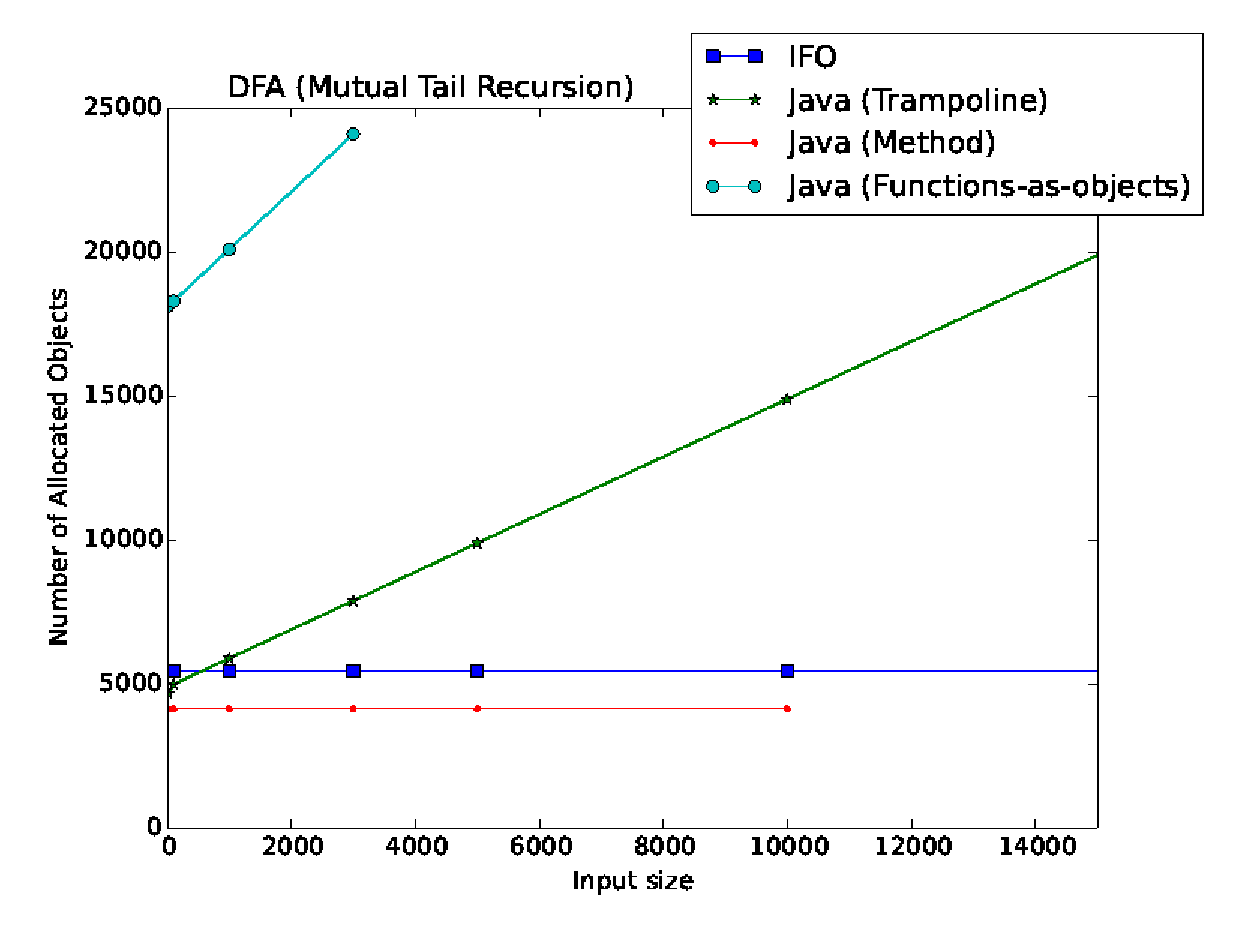
\includegraphics[width=7cm]{./src/img/dfa2an.eps}}\end{minipage} 
\end{tabular} 
 
 
 



\end{center}
\vspace{-15pt}
\caption{The DFA encoding: the two columns show the minimum and maximum numbers of total allocated objects on heap from isolated profiled runs with all input lengths. Due to space limitations, the x-axes of plots are cropped at 15000 for clarity.}

\label{fig:dfa}
\end{figure}

One common idiom in functional programming is encoding finite states
as tail recursive functions and state transitions as mutual calls
among these functions. One trivial example of this is the naive
even-odd program which switches between two states. A more useful
application is in the implementation of finite state automata
\cite{Krishnamurthi2006}. Normally, functional language programmers
seek this idiom for its conciseness. However in JVM-hosted functional
languages, programmers tend to avoid this idiom, because they either
lose correctness (\lstinline{StackOverflow} exceptions in a
method-based representation) or performance (in a trampoline-based
one). In this experiment, we implemented a DFA recognizing a regular
expression $(AAB^{*}|A^{*}B)^{+}$ and measured the performance on
randomly generated Strings with different lengths.

We implemented it in \name to assess
IFOs (with all the optimizations mentioned in Sections \ref{sec:tce} and
\ref{sec:implementation}) and in Java (1.8.0\_25) to assess different closure representations: method
calls, Java 8's lambdas (functions-as-objects), and custom
trampolines. We chose plain Java implementation, because we can examine the
runtime behavior of different representations without potential
compiler overheads. All implementations used primitive \lstinline{char} variables and did not allocated any
new objects on heap when reading from the input Strings.
We report the total number of allocated objects on heap in the isolated application
runs, as measured by HPROF~ \cite{hprof}, the JDK's profiling tool.

\noindent We executed all benchmarks on the following platform with
the HotSpot\texttrademark VM (1.8.0\_25):
Intel\textregistered Core\texttrademark i5 3570 CPU, 1600MHz DDR3 4GB
RAM, Ubuntu 14.04.1.

We show the result of this experiment in Figure \ref{fig:dfa}. The IFO-
and trampoline-based implementations continued executing after method-based and FAO-based
ones threw a \lstinline{StackOverflow} exception. IFOs, similarly
to the method-based implementation, allocated a constant number of
objects on heap. The trampoline one, however, increased its object
allocation with the input, because it needed to create an object for 
each tail call.
\subsubsection{Time Overhead: Isolated Call Behavior.}\label{sec:micro}
\begin{figure}[h!t]
 \begin{center} 
\begin{tabular}{|l|l|l|l|l|}
\hline
\multicolumn{1}{|r|}{\textit{\textbf{Low Input Values}}} & fact(20) in $ns$           & fib(20) in $ns$           & tailfact(20) in $ns$      & evenodd(256) in $\mu s$           \\ \hline
\textbf{IFO}                                      & $204.84 \pm 2.35$   & $35.50 \pm 0.47$   & $49.52 \pm 0.72$  & $32.95 \pm 0.09$    \\ \hline
\textbf{Java}                                     & $147.95 \pm 0.65$   & $22.50 \pm 0.06$   & $18.18 \pm 0.19$  & $30.93 \pm 0.12$   \\ \hline
\textbf{Java (T)}                                 & $1280.23 \pm 20.99$ & $502.35 \pm 9.42$ & $139.39 \pm 1.79$ & $474.41 \pm 6.29$ \\ \hline
\textbf{Scala}                                    & $130.46 \pm 0.40$    & $22.55 \pm 0.14$  & $15.94 \pm 0.05$  & $32.79 \pm 0.09$    \\ \hline
\textbf{Clojure}                                  & $573.95 \pm 3.41$   & $314.24 \pm 2.25$ & $205.21 \pm 0.35$ & $82.61 \pm 0.95$   \\ \hline
\end{tabular}

\begin{tabular}{|l|l|l|}
\hline
\multicolumn{1}{|r|}{\textit{\textbf{High Input Values}}}  & evenodd(214748) in $\mu s$ & tailfact(10000) in $\mu s$ \\ \hline
\textbf{IFO}                                                                                               & $152.47 \pm 0.43$     & $166.64 \pm 0.51$    \\ \hline
\textbf{Java}                                                                                              & $1060.35 \pm 14.52$ & $644.10 \pm 3.89$   \\ \hline
\textbf{Scala}                                                                                              & $1864.34 \pm 31.24$  & $1004.13 \pm 13.49$ \\ \hline
\textbf{Clojure}                                                                                           & $6533.14 \pm 92.65$ & N/A                       \\ \hline
\end{tabular}
  \begin{tabular}{ll}
  \begin{minipage}{6.2cm}{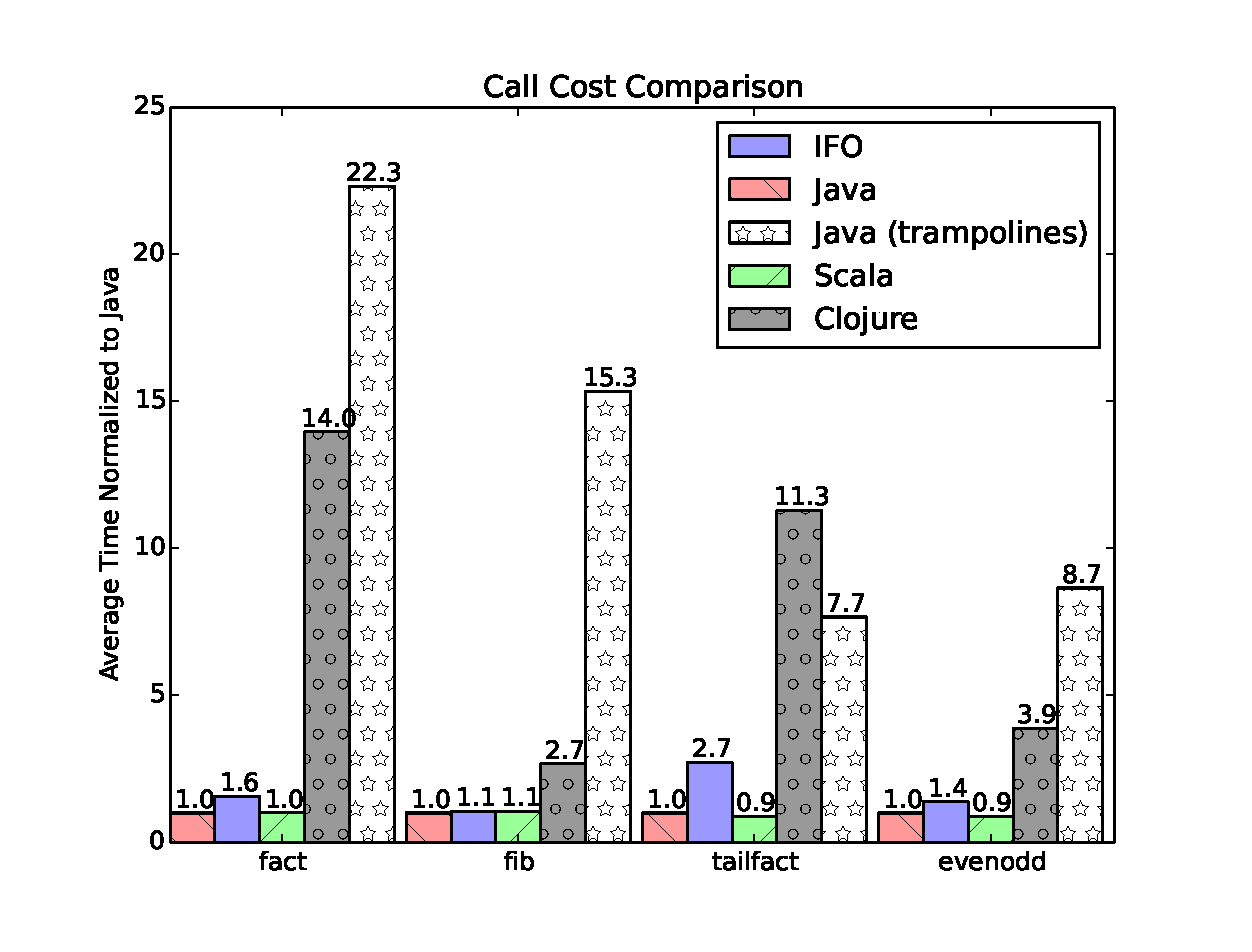
\includegraphics[width=6.2cm]{./src/img/low.eps}}\end{minipage} &
\begin{minipage}{6.2cm}{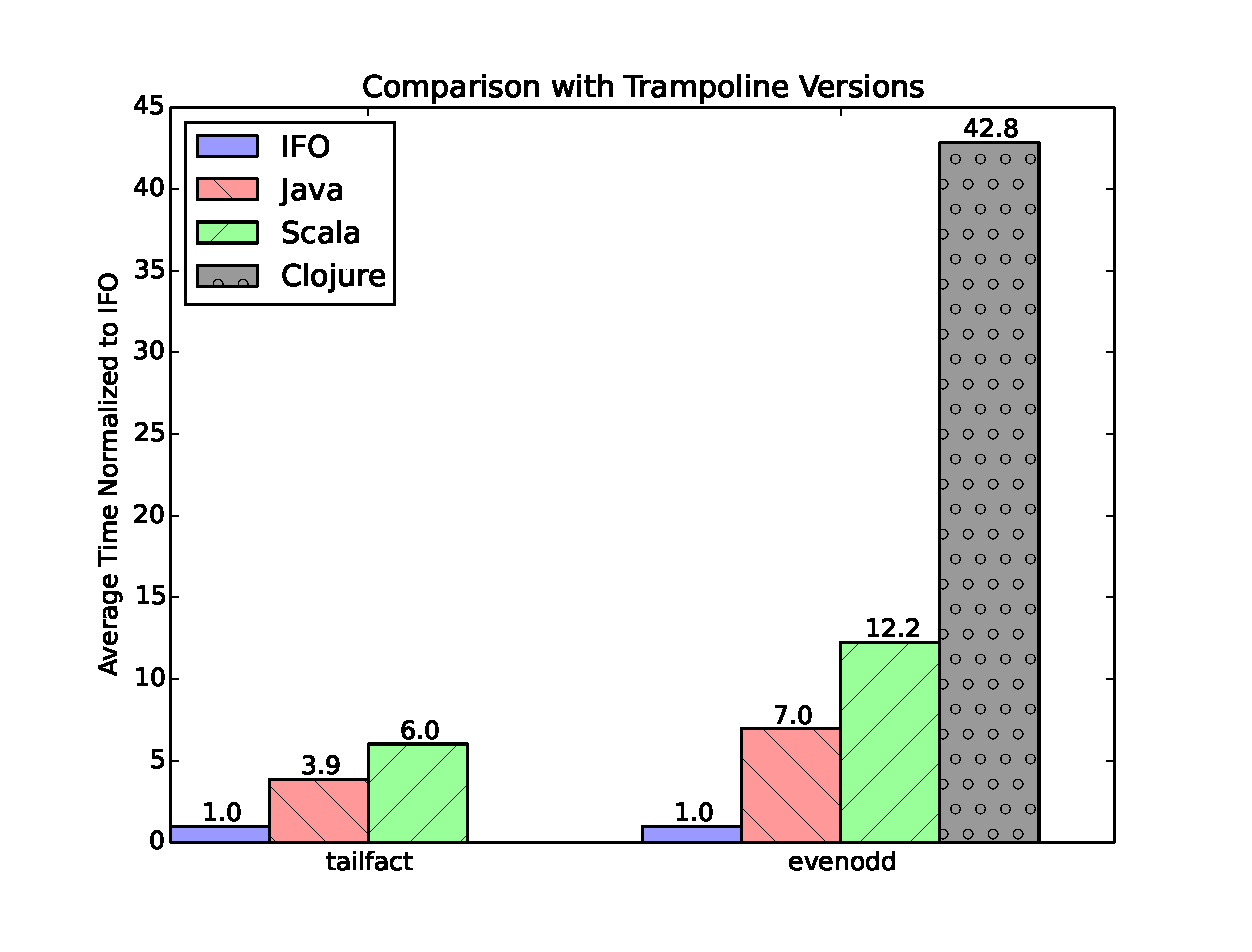
\includegraphics[width=6.2cm]{./src/img/high.eps}}\end{minipage}
\end{tabular}

\end{center}
\vspace{-20pt}
  \caption{The isolated call behavior experiments: the reported times are averages of 10 measured runs and corresponding standard deviations. The plots are normalized to Java's (left table and plot) and IFO's (right table and plot) results -- the lower, the faster.}

\label{fig:micro}
\end{figure}
For measuring time overhead, we show two experiments: isolated simple call behavior in 
different microbenchmarks and the time performance of the DFA implementation.
We wrote the benchmark programs in the extended System F for our
compilation process and in the following JVM-hosted languages in their
stable versions: \emph{Scala} (2.11.2)\cite{Odersky2014b}, 
\emph{Clojure} (1.6.0)\cite{Hickey2008}, and Java (1.8.0\_25, as before).
For encoding mutually recursive tail calls, we used the provided trampoline 
facilities in Scala (\texttt{scala.util.control .TailCalls}) and
Clojure (\texttt{tramp} from \texttt{clojure.core.logic}).

\noindent The programs were executed on the same platform as the memory experiment.
For the automation of performance measurement, we used the
Java Microbenchmark Harness (JMH) tool which is a part of OpenJDK
\cite{jmh}. Based on the provided annotations, JMH measures execution
of given programs. In addition to that, it takes necessary steps to
gain stable results. They include non-measured warm-up iterations for
JITC, forcing garbage collection before each benchmark, and running
benchmarks in isolated VM instances. We configured JMH for 10 warm-up
runs and 10 measured runs from which we compute averages.

We chose four programs to represent the following behaviors:
\begin{itemize}

  \item \emph{Non-tail recursive calls}: Computing the factorial and
    Fibonacci numbers using naive algorithms.

  \item \emph{Single method tail recursive calls}: Computing factorial
    using a tail recursive implementation.

  \item \emph{Mutually recursive tail calls}: Testing evenness and
    oddness using two mutually recursive functions.
\end{itemize}
\noindent Non-tail recursive programs present two examples of general
recursive calls and we executed them, altogether with the tail
recursive programs, on low input values (not causing
\lstinline{StackOverflow} exceptions in default JVM settings). In
addition to that, we executed the tail recursive programs on high input
values in which method-based implementations threw
\lstinline{StackOverflow} exceptions in default JVM settings. We show the results in Figure \ref{fig:micro}. Its left part shows
the result for low input values in IFOs, method implementations in all
the other languages and the fastest trampoline implementation (Java);
the plot is normalized to the Java method-based
implementation's results. The right part shows the result for high input values
in IFO- and trampoline-based implementations; the plot is normalized to results of 
IFO-based implementations. For low input values, we can see that IFO-based implementations run
slightly slower than method-based ones. However, their overhead is
small compared with the fastest trampoline implementations in our
evaluation. IFOs ran 0.1 to 1.7-times slower than method-based
representations, whereas the fastest trampolines ran 7.7 to 22.3-times
slower. In the tail recursive programs, Scala ran slightly faster than
standard Java methods due to its compiler optimizations. Clojure has
an additional overhead, because its compiler enforces integer overflow
checking. For the high input values, the method-based implementations threw a
\lstinline{StackOverflow} exception in default JVM settings, unlike
IFOs and trampoline implementations which can continue executing with
this input. IFOs ran 3.9 to 12.2-times faster (excluding Clojure) than
trampoline implementations. Again, Clojure suffered from its
additional overhead and threw an integer overflow exception in the
tail recursive factorial. Using BigIntegers would prevent this, but
we wanted to isolate the call behavior in this experiment, i.e. avoid
any extra overhead from other object allocations.
\subsubsection{Time Overhead: DFA Performance.}
\begin{figure}[h!t]
\vspace{10pt}
 \begin{center} 
 
\begin{tabular}{|l|l|l|l|l|}
\hline
\multicolumn{1}{|r|}{\textit{\textbf{Input length (time unit)}}} & 1000 ($\mu s$)                 & 3000 ($\mu s$)                  & 10000 ($\mu s$)                   & 100000 ($\mu s$)                 \\ \hline
\textbf{IFO}                                  & $5.10 \pm 0.10$   & $15.98 \pm 0.07$  & $77.81 \pm 0.83$   & $933.58 \pm 13.40$      \\ \hline
\textbf{Java (Trampoline-based)}                             & $7.03 \pm 0.130$ & $26.89 \pm 0.10$ & $102.98 \pm 2.36$ & $1099.80 \pm 15.46$ \\ \hline
\textbf{Java (Method-based)}                             & $3.80 \pm 0.07$  & $11.61 \pm 0.10$  & $48.83 \pm 0.13$    & N/A                        \\ \hline
\textbf{Java (FAO-based)}                           & $6.37 \pm 0.01$   & $17.62 \pm 0.05$  & N/A                     & N/A                       \\ \hline
\end{tabular}

\begin{minipage}{10cm}{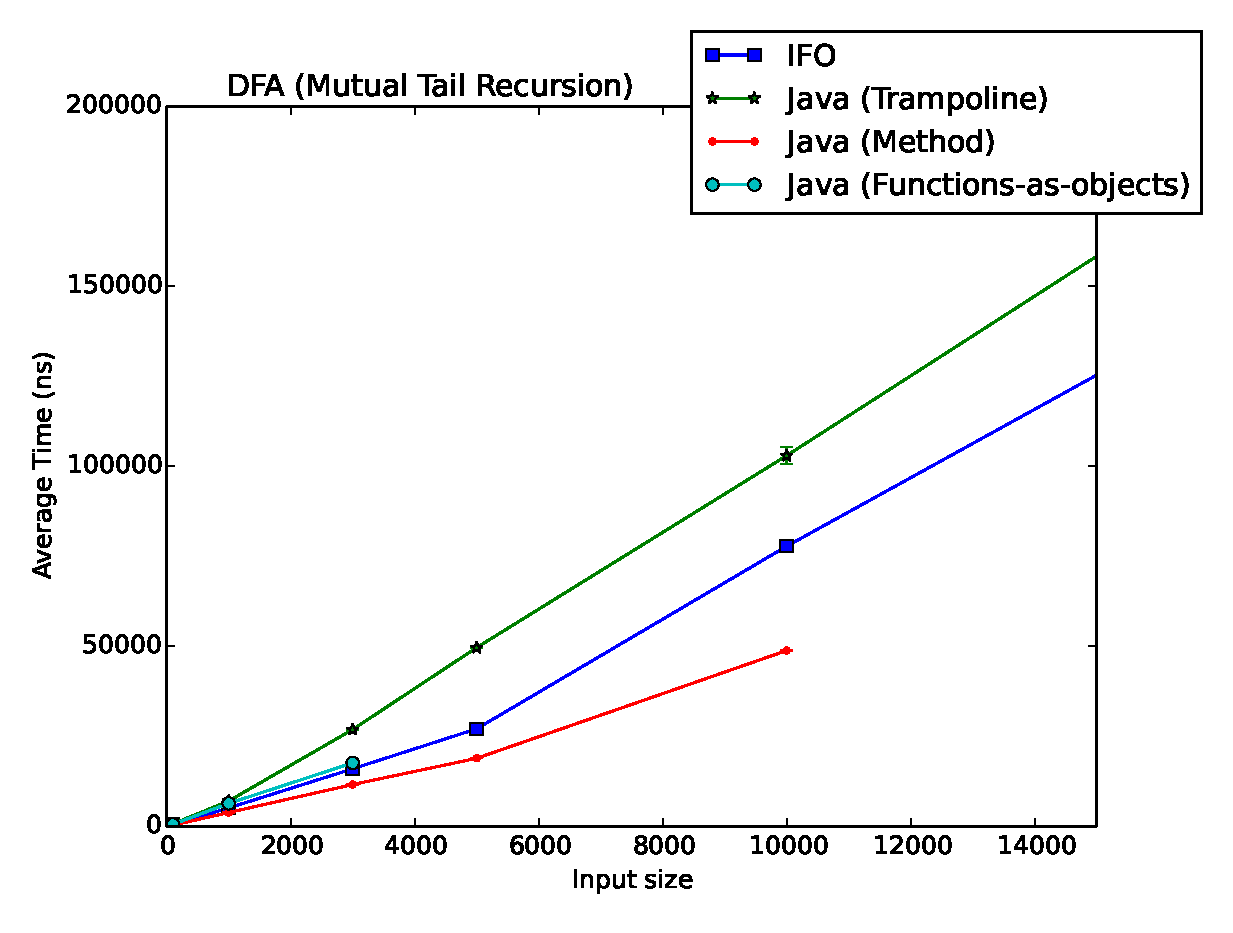
\includegraphics[width=10cm]{./src/img/dfa1.eps}}\end{minipage} 

\end{center}
\vspace{-15pt}
\caption{The DFA encoding: the reported times are averages of 10 measured runs and corresponding standard deviations. Due to space limitations, the x-axes of plots are cropped at 15000 for clarity.}

\label{fig:dfa2}
\end{figure}
Unlike the first experiment, where
the programs isolated costs of plain recursive calls, DFA encoding 
represents a more realistic behavior with other costs, such as
non-recursive method calls and calls to other API methods (e.g. reading input).
The setting was the same as in the constant memory experiment 
and we performed time measurement in the same way as in the isolated call behavior experiment. We show the result of this experiment in Figure \ref{fig:dfa2}. The
FAO-based implementation ran slowest out of all implementations and threw
\lstinline{StackOverflow} exception with a smaller input than the
method-based implementation. That is because it creates extra objects
and performs extra calls due to its representation. As in the isolated
calls experiment, the IFO-based implementation ran about 0.5-times slower than method-based
implementation. Trampolines, however, ran about 2-times slower. The IFO-
and trampoline-based implementations continued executing after method-based
one threw a \lstinline{StackOverflow} exception. The IFO-based
implementation was about 0.2-times faster than the trampoline one for 
larger inputs.